\documentclass[12pt,a4paper]{article}

% =========================================================================
% GÓI THƯ VIỆN & CẤU HÌNH CƠ BẢN (XELATEX COMPATIBLE)
% =========================================================================
\usepackage{fontspec}
\setmainfont{Times New Roman}

\usepackage[top=2.2cm, bottom=2.2cm, left=2.5cm, right=2.0cm]{geometry}
\usepackage{amsmath, amsfonts, amssymb}
\usepackage{graphicx}
\usepackage{booktabs}
\usepackage{tabularx}
\usepackage{array}
\usepackage{float}
\usepackage{xcolor}
\usepackage{colortbl}
\usepackage{tikz}
\usetikzlibrary{calc, shapes.geometric, arrows.meta, positioning}
\usepackage{hyperref}
\usepackage{fancyhdr}
\usepackage{titlesec}
\usepackage{caption}
\usepackage{subcaption}
\usepackage{enumitem}
\usepackage{listings}
\usepackage{setspace}

% Dãn dòng chuẩn học thuật PTIT
\setstretch{1.2}

% Định nghĩa màu sắc thương hiệu báo cáo
\definecolor{ptitblue}{RGB}{0, 51, 153}
\definecolor{darkblue}{RGB}{10, 40, 100}
\definecolor{lightgray}{RGB}{245, 247, 250}

% Cấu hình Tiếng Việt cho Caption
\renewcommand{\figurename}{Hình}
\renewcommand{\tablename}{Bảng}
\captionsetup[figure]{name=Hình, labelfont={bf,color=blue!70!black}, font=small, skip=4pt}
\captionsetup[table]{name=Bảng, labelfont={bf,color=blue!70!black}, font=small, skip=4pt}

% Cấu hình Hyperref
\hypersetup{
    colorlinks=true,
    linkcolor=blue!80!black,
    citecolor=green!60!black,
    urlcolor=blue!70!black,
    pdftitle={Báo cáo Bài tập Agent 01: Discovering AI Agents & Reinforcement Learning},
    pdfauthor={Phạm Văn Tư - B23DCCN879}
}

% Định dạng tiêu đề mục
\titleformat{\section}
  {\normalfont\Large\bfseries\color{blue!70!black}}
  {\thesection}{1em}{}
\titlespacing*{\section}{0pt}{8pt}{4pt}

\titleformat{\subsection}
  {\normalfont\large\bfseries\color{black!85}}
  {\thesubsection}{1em}{}
\titlespacing*{\subsection}{0pt}{6pt}{3pt}

% Danh sách gọn gàng
\setlist[itemize]{leftmargin=1.5em, itemsep=1.5pt, topsep=2pt, parsep=0pt}
\setlist[enumerate]{leftmargin=1.5em, itemsep=1.5pt, topsep=2pt, parsep=0pt}

% Header & Footer
\pagestyle{fancy}
\fancyhf{}
\fancyhead[R]{\small\itshape Báo cáo Bài tập Agent 01: Discovering AI Agents}
\fancyfoot[C]{\thepage}
\renewcommand{\headrulewidth}{0.4pt}
\setlength{\headheight}{14pt}

\begin{document}

% -------------------------------------------------------------------------
% TRANG BÌA CHUẨN HỌC VIỆN CÔNG NGHỆ BƯU CHÍNH VIỄN THÔNG
% -------------------------------------------------------------------------
\begin{titlepage}
\begin{tikzpicture}[remember picture, overlay]
    \node[anchor=center] at (current page.center) {
        
\includegraphics[width=\dimexpr\paperwidth-2.0cm\relax, height=\dimexpr\paperheight-2.0cm\relax]{images/ptit_cover_border.jpeg}
    };
\end{tikzpicture}

\begin{center}
    \vspace*{-0.2cm}
    {\fontsize{14.5pt}{19pt}\selectfont \textbf{HỌC VIỆN CÔNG NGHỆ BƯU CHÍNH VIỄN THÔNG}}\\[0.3cm]
    {\fontsize{14.5pt}{19pt}\selectfont \textbf{KHOA CÔNG NGHỆ THÔNG TIN 1}}\\[0.3cm]
    {\fontsize{14.5pt}{19pt}\selectfont \textbf{HỌC PHẦN PHÁT TRIỂN CÁC HỆ THỐNG THÔNG MINH}}\\[1.1cm]
    
    % Logo PTIT
    
\includegraphics[width=4.3cm]{images/ptit_logo.png}\\[1.3cm]
    
    {\fontsize{18pt}{23pt}\selectfont \textbf{BÁO CÁO BÀI TẬP (AGENT 01)}}\\[0.4cm]
    {\fontsize{14pt}{19pt}\selectfont \textbf{TÌM HIỂU VỀ HỆ TÁC TỬ THÔNG MINH (AI AGENT)}}\\[0.2cm]
    {\fontsize{13pt}{18pt}\selectfont \textbf{VÀ TÁC TỬ HỌC TĂNG CƯỜNG (REINFORCEMENT LEARNING)}}\\[1.4cm]
\end{center}

\begin{flushleft}
    \hspace{2.8cm}
    \begin{tabular}{ll}
        \textbf{Lớp:} & D23CTPM01 \\[0.3cm]
        \textbf{Họ và tên:} & Phạm Văn Tư \\[0.3cm]
        \textbf{Mã sinh viên:} & B23DCCN879 \\[0.3cm]
        \textbf{Giảng viên hướng dẫn:} & PGS.TS Trần Đình Quế \\[0.3cm]
        \textbf{Học kỳ:} & Học kỳ 1 năm học 2026 – 2027
    \end{tabular}
\end{flushleft}

\vfill
\begin{center}
    {\fontsize{12pt}{15pt}\selectfont \textbf{Hà Nội, 2026}}\\[0.4cm]
\end{center}
\end{titlepage}

\clearpage
\pagenumbering{arabic}

% =========================================================================
% TRANG 1 NỘI DUNG: MỞ ĐẦU & BẢN CHẤT 3 TRỤ CỘT (GOOGLE CLOUD [1] & MCKINSEY [3])
% =========================================================================

\section*{LỜI MỞ ĐẦU VÀ TỔNG QUAN BÀI TẬP}

Trong kỷ nguyên bùng nổ của Trí tuệ nhân tạo (AI), sự xuất hiện của các Mô hình ngôn ngữ lớn (LLMs) đã tái định hình năng lực xử lý ngôn ngữ tự nhiên. Tuy nhiên, các mô hình nền tảng chỉ phản hồi thụ động (\textit{prompt-and-response}), bị đóng băng tri thức và không thể trực tiếp thao tác vào môi trường số. Nhằm vượt qua ranh giới này, một bước chuyển dịch mang tính đột phá đang diễn ra: sự xuất hiện của \textbf{Hệ tác tử thông minh (Artificial Intelligence Agents / Agentic AI)}. Dựa trên các tài liệu công nghệ hàng đầu thế giới được chỉ định nghiên cứu bao gồm: \textbf{Google Cloud [1]}, \textbf{IBM Think [2]} và \textbf{McKinsey [3]}, báo cáo này trình bày sự hiểu biết toàn diện về AI Agent, đồng thời cung cấp minh chứng thực nghiệm xây dựng Tác tử Học tăng cường (Q-Learning Agent) giải bài toán điều hướng mê cung trên môi trường Jupyter Notebook dựa trên tài liệu \textbf{GeeksforGeeks [4]}.

\section{BẢN CHẤT VÀ BA TRỤ CỘT NỀN TẢNG CỦA AI AGENT}

\subsection{Định nghĩa học thuật theo Google Cloud và McKinsey}
Theo tài liệu \textbf{Google Cloud [1]} và \textbf{McKinsey [3]}, AI Agent là hệ thống phần mềm được vận hành bởi các mô hình Generative AI, sở hữu mức độ tự trị để chủ động theo đuổi mục tiêu và hoàn thành các chuỗi tác vụ phức hợp thay mặt cho người dùng. Một tác tử thông minh tiêu chuẩn được xây dựng trên 3 trụ cột kỹ thuật: (1) \textbf{Suy luận và Lập kế hoạch (Reasoning \& Planning)} phân rã mục tiêu lớn thành chuỗi tác vụ con tuần tự và tối ưu; (2) \textbf{Bộ nhớ và Quản lý Ngữ cảnh (Memory Management)} gồm bộ nhớ ngắn hạn duy trì hội thoại và bộ nhớ dài hạn tra cứu qua Vector DB / Knowledge Graph; và (3) \textbf{Sử dụng Công cụ Ngoại vi (Tool Use \& Action Engine)} chủ động kích hoạt Function Calling, truy vấn CSDL nội bộ và thực thi mã lệnh tạo tác động thực tế.

\begin{figure}[H]
    \centering
    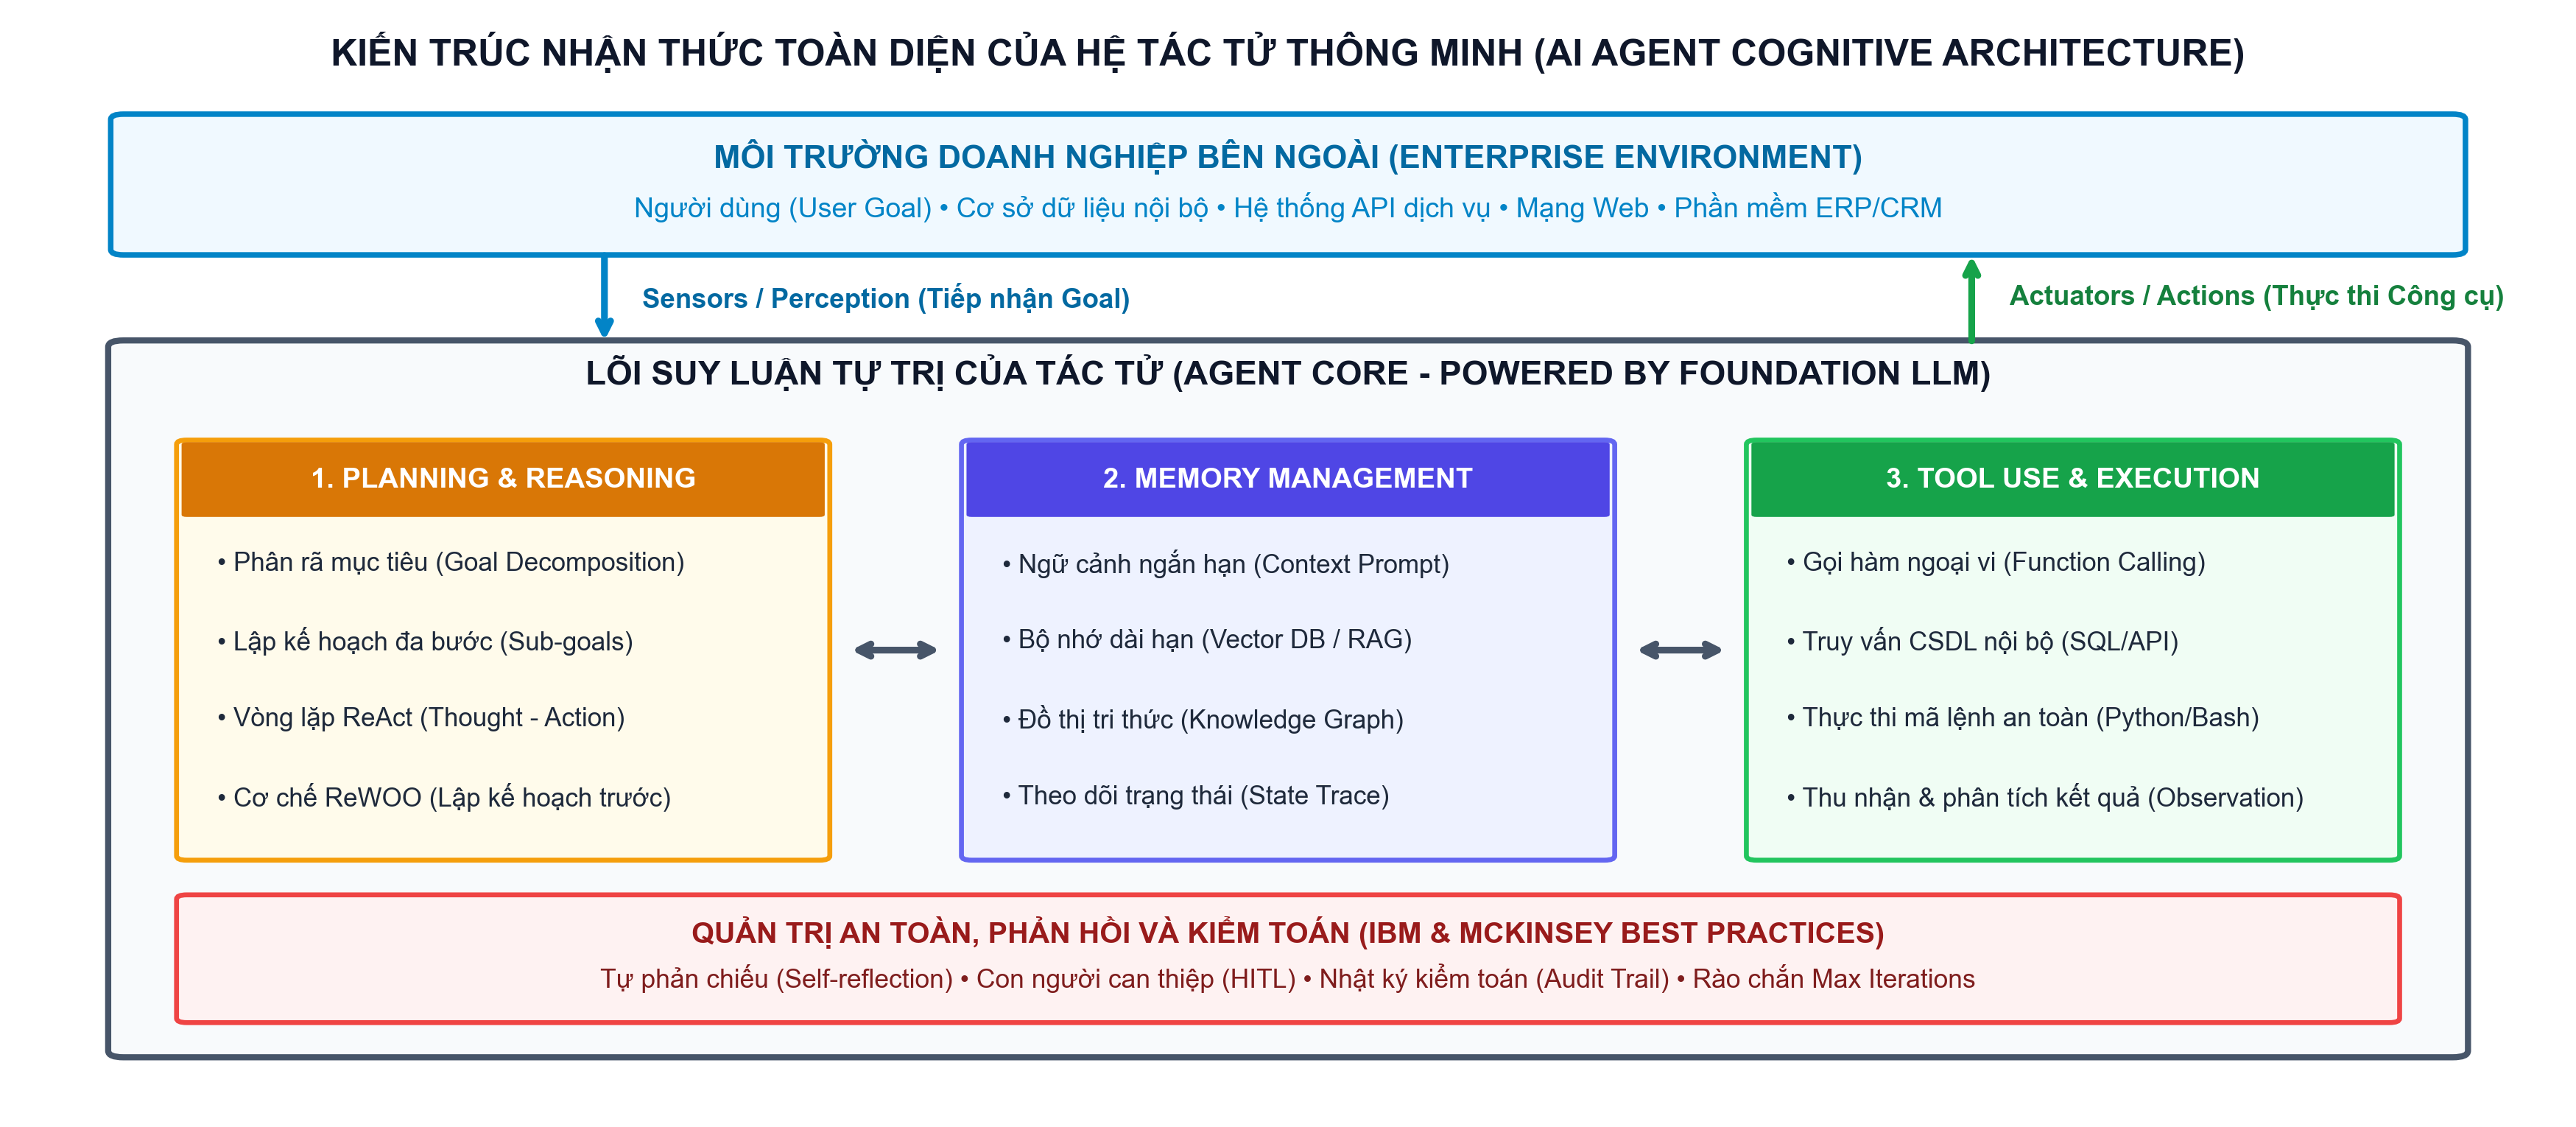
\includegraphics[width=0.96\textwidth]{images/fig_ai_agent_architecture.png}
    \caption{Sơ đồ kiến trúc nhận thức toàn diện của một Hệ tác tử thông minh (AI Agent Cognitive Architecture).}
    \label{fig:ai_agent_architecture}
\end{figure}

\clearpage

% =========================================================================
% TRANG 2 NỘI DUNG: SỰ TIẾN HÓA MÔ HÌNH: CHATBOT ĐẾN AGENTIC MESH (MCKINSEY [3])
% =========================================================================

\section{SỰ TIẾN HÓA MÔ HÌNH: TỪ CHATBOT ĐẾN AGENTIC MESH}

\subsection{Đối sánh toàn diện: Non-agentic Chatbot vs. AI Copilot vs. Autonomous Agent}
Để làm rõ sự khác biệt căn bản về bản chất kỹ thuật, Bảng~\ref{tab:comparison} đối sánh ba thế hệ công nghệ dựa trên các tiêu chí vận hành được tổng hợp từ Google Cloud [1] và McKinsey [3].

\begin{table}[H]
\centering
\footnotesize
\caption{Bảng đối sánh giữa Chatbot truyền thống, Trợ lý AI Copilot và Hệ tác tử tự trị.}
\label{tab:comparison}
\begin{tabularx}{\textwidth}{@{} l X X X @{}}
\toprule
\textbf{Tiêu chí đánh giá} & \textbf{Non-agentic Chatbot} & \textbf{AI Copilot (Trợ lý)} & \textbf{Autonomous AI Agent} \\
\midrule
\textbf{Mức độ tự trị} & Thụ động, 100\% dựa vào prompt & Hỗ trợ người dùng từng bước & Tự trị cao, tự điều hướng mục tiêu \\
\textbf{Lập kế hoạch} & Không có cơ chế lập kế hoạch & Con người tự lập kế hoạch & Tự phân rã nhiệm vụ đa bước \\
\textbf{Sử dụng công cụ} & Không có hoặc rất hạn chế & Con người xác nhận từng lệnh gọi & Tự động lựa chọn và thực thi công cụ \\
\textbf{Quản lý bộ nhớ} & Cửa sổ ngữ cảnh phiên ngắn & Ngữ cảnh theo phiên làm việc & Bộ nhớ dài hạn, lưu vết trạng thái \\
\textbf{Cơ chế sửa sai} & Không thể tự sửa lỗi & Phụ thuộc vào phản hồi người dùng & Tự phản chiếu (Self-reflection), thử lại \\
\textbf{Vai trò con người} & Đặt câu hỏi và đọc kết quả & Thao tác chính, AI gợi ý & Giám sát cấp cao (Supervisor / HITL) \\
\bottomrule
\end{tabularx}
\end{table}

\subsection{Lộ trình 4 giai đoạn tiến hóa công nghệ trong tổ chức}
Hình~\ref{fig:evolution_mesh} minh họa lộ trình chuyển dịch tất yếu của Trí tuệ nhân tạo trong môi trường doanh nghiệp: từ các Chatbot thụ động (Giai đoạn 1), qua Trợ lý Copilot (Giai đoạn 2), Tác tử đơn lẻ tự trị (Giai đoạn 3), và hướng tới Mạng lưới tác tử doanh nghiệp đa năng (\textit{Agentic Mesh} -- Giai đoạn 4).

\begin{figure}[H]
    \centering
    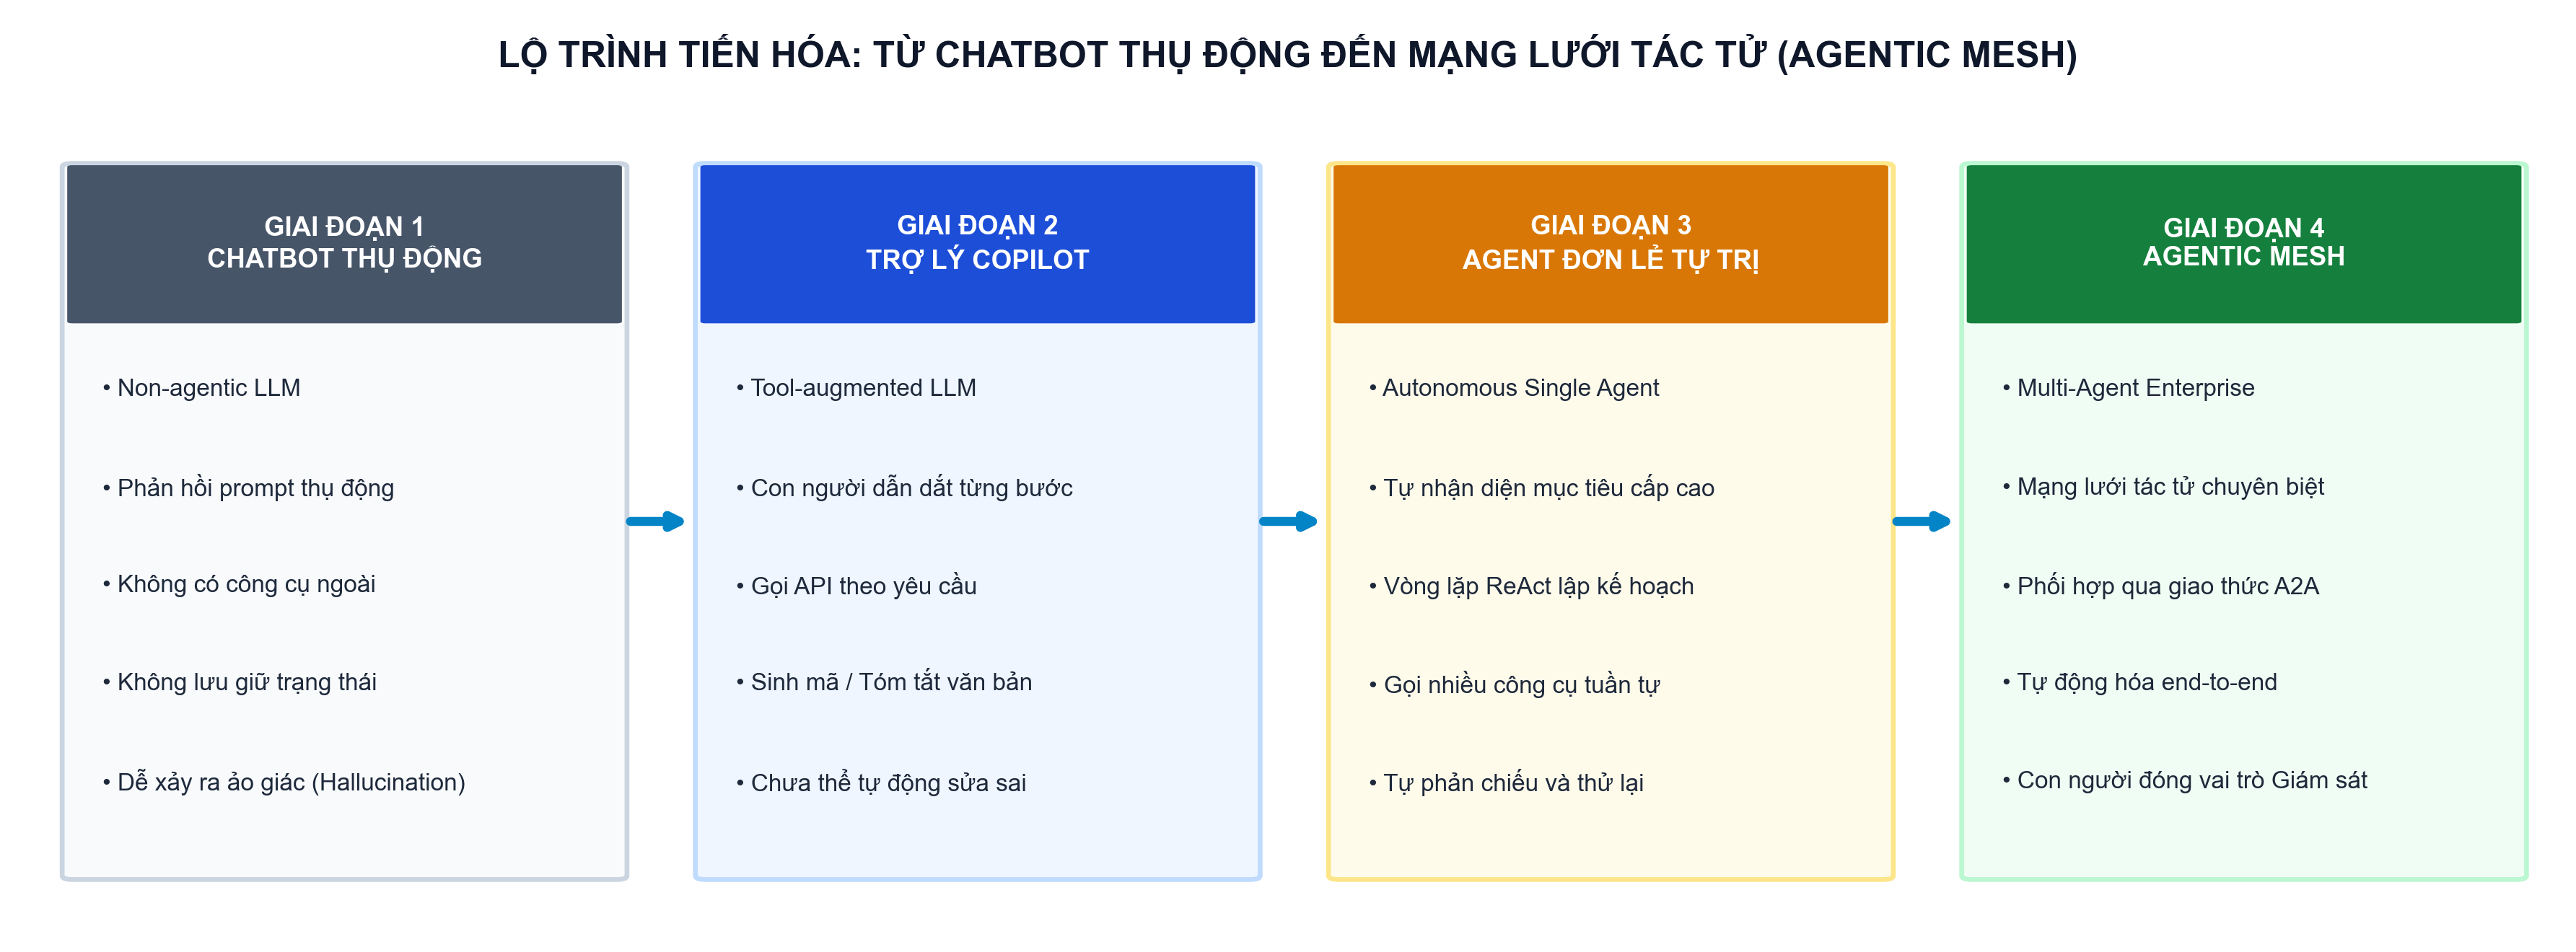
\includegraphics[width=0.96\textwidth]{images/fig_evolution_mesh.png}
    \caption{Lộ trình tiến hóa công nghệ từ Chatbot thụ động đến Mạng lưới tác tử doanh nghiệp (Agentic Mesh).}
    \label{fig:evolution_mesh}
\end{figure}

\subsection{Nguyên lý Mạng lưới Tác tử (Agentic Mesh) theo McKinsey}
Khái niệm \textbf{Agentic Mesh} do McKinsey [3] đề xuất biểu trưng cho một mạng lưới các tác tử chuyên môn hóa sâu, phối hợp với nhau qua các giao thức tương tác (Agent-to-Agent communication) để vận hành các quy trình nghiệp vụ phức hợp mà không cần sự can thiệp thủ công liên tục của con người.

\clearpage

% =========================================================================
% TRANG 3 NỘI DUNG: KIẾN TRÚC KỸ THUẬT VÀ CƠ CHẾ SUY LUẬN (IBM THINK [2])
% =========================================================================

\section{KIẾN TRÚC KỸ THUẬT VÀ CƠ CHẾ SUY LUẬN THEO IBM THINK}

\subsection{Chu trình nhận thức ba giai đoạn (IBM Cognitive Cycle)}
Tài liệu của \textbf{IBM Think [2]} phân tích sâu sắc cơ chế hoạt động của AI Agent qua chu trình 3 giai đoạn khép kín: (1) \textbf{Khởi tạo mục tiêu và Lập kế hoạch (Goal Initialization \& Planning)} phân rã yêu cầu thành các hành động đo lường được; (2) \textbf{Suy luận kết hợp Công cụ ngoại vi (Reasoning with Available Tools)} nhận thức môi trường và gọi công cụ bổ sung tri thức thực tế; và (3) \textbf{Học hỏi và Tự phản chiếu (Learning \& Reflection)} phân tích kết quả phản hồi và tinh chỉnh lại kế hoạch (\textit{iterative refinement}) nếu gặp lỗi.

\subsection{Đối chiếu chuyên sâu hai mô hình suy luận: ReAct vs. ReWOO}
IBM Think [2] chỉ rõ hai trường phái suy luận then chốt định hình hiệu năng của tác tử:
\begin{itemize}[itemsep=1pt,topsep=2pt]
    \item \textbf{Mô hình ReAct (Reasoning and Action):} Vận hành theo vòng lặp đan xen: \textit{Suy nghĩ (Thought)} $\to$ \textit{Hành động (Action)} $\to$ \textit{Quan sát kết quả (Observation)}. Thích ứng rất linh hoạt nhưng độ trễ cao và tiêu tốn nhiều token do phải gọi LLM sau mỗi bước quan sát.
    \item \textbf{Mô hình ReWOO (Reasoning Without Observation):} Tách rời pha lập kế hoạch và thực thi thành 3 module: \textit{Planner} (lập trước toàn bộ đồ thị gọi công cụ), \textit{Worker} (gọi song song API ngoại vi), và \textit{Solver} (tổng hợp dữ liệu). Tiết kiệm tối đa chi phí token và giảm triệt để độ trễ.
\end{itemize}

\begin{figure}[H]
    \centering
    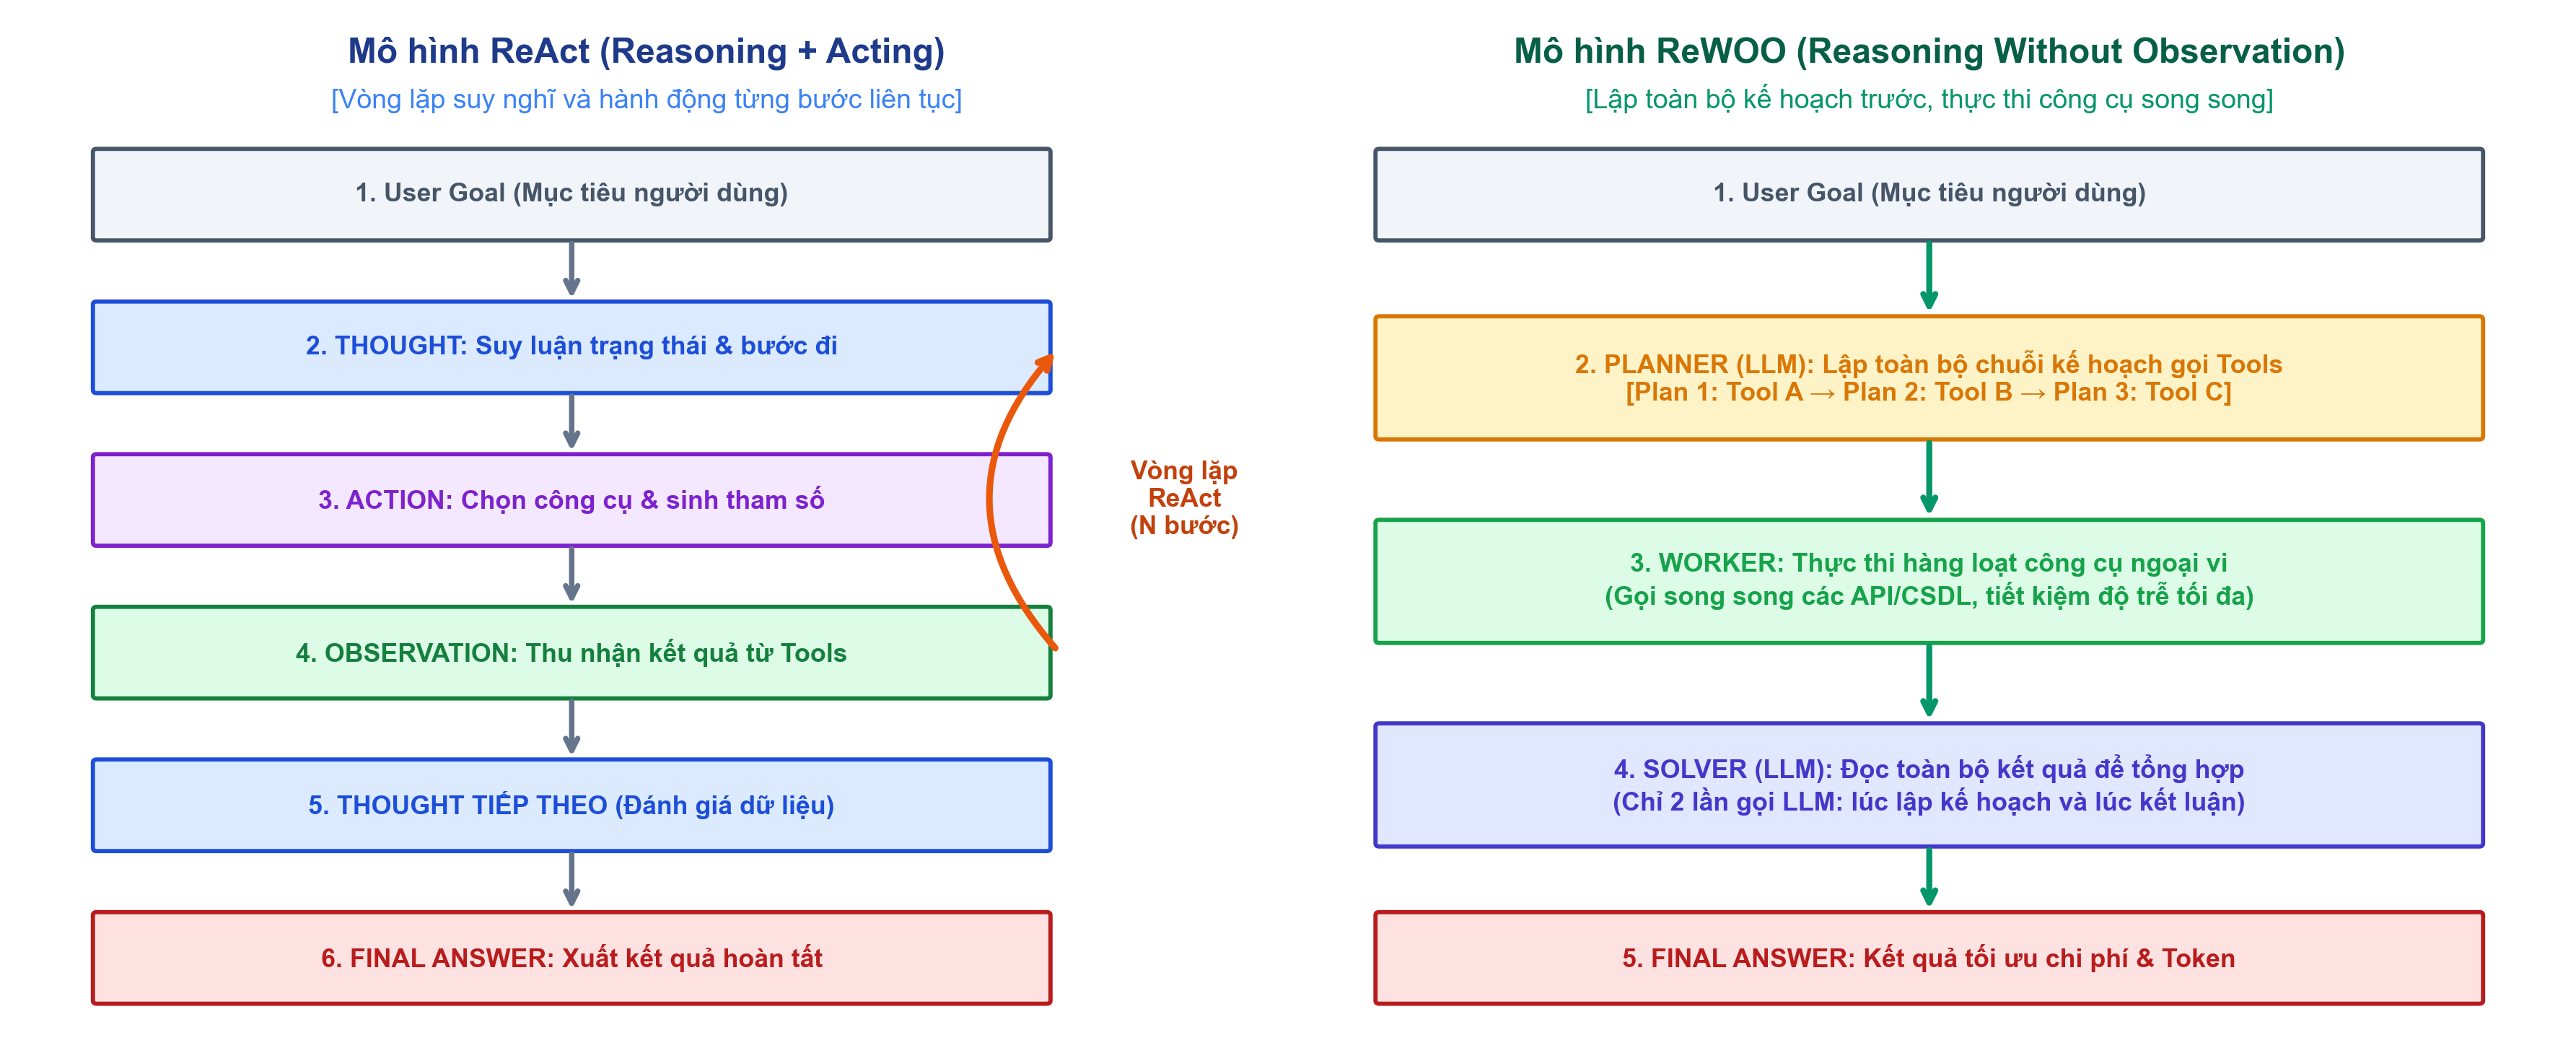
\includegraphics[width=0.95\textwidth]{images/fig_react_vs_rewoo.png}
    \caption{So sánh cơ chế vận hành giữa mô hình ReAct (vòng lặp liên tục) và ReWOO (lập kế hoạch trước và thực thi song song).}
    \label{fig:react_vs_rewoo}
\end{figure}

\subsection{Các mô hình suy luận nâng cao khác}
Ngoài ReAct và ReWOO, các tác tử hiện đại còn áp dụng mô hình \textbf{Plan-and-Solve} (lập kế hoạch trừu tượng trước khi chi tiết hóa), \textbf{LLM Compiler} (tối ưu hóa luồng thực thi phụ thuộc song song) và \textbf{Reflection} (tác tử phản biện độc lập để rà soát lỗi trước khi hoàn tất).

\clearpage

% =========================================================================
% TRANG 4 NỘI DUNG: PHÂN CẤP TÁC TỬ KINH ĐIỂN VÀ MÔ HÌNH HỌC MÁY (RUSSELL & NORVIG)
% =========================================================================

\section{NĂM PHÂN CẤP TÁC TỬ KINH ĐIỂN VÀ MÔ HÌNH HỌC MÁY}

\subsection{Năm phân cấp tác tử kinh điển theo Russell \& Norvig}
Tài liệu \textbf{IBM Think [2]} quy chiếu các kiến trúc tác tử hiện đại về 5 cấp độ tác tử kinh điển của Russell \& Norvig [6]: (1) \textbf{Simple reflex agents} (phản xạ trực tiếp theo luật điều kiện--hành động, không lưu vết); (2) \textbf{Model-based reflex agents} (duy trì mô hình trạng thái nội tại xử lý môi trường quan sát một phần); (3) \textbf{Goal-based agents} (ra quyết định dựa trên mục tiêu định trước và tìm kiếm đường đi); (4) \textbf{Utility-based agents} (tối ưu hóa hàm hữu dụng khi có nhiều phương án cạnh tranh); và (5) \textbf{Learning agents} (tác tử học máy tự cải thiện năng lực qua tương tác và phản hồi môi trường).

\subsection{Cấu trúc nội tại của Tác tử Học máy (Learning Agent Architecture)}
Theo Russell \& Norvig [6], một \textit{Learning Agent} chuẩn mực gồm 4 thành phần chức năng tương hỗ: \textbf{Critic} (đối chiếu hành vi với tiêu chuẩn hiệu năng để sinh tín hiệu phản hồi), \textbf{Learning Element} (tiếp nhận phản hồi cập nhật chính sách), \textbf{Performance Element} (chọn hành động thực thi vào môi trường), và \textbf{Problem Generator} (đề xuất hành vi thăm dò mới tích lũy kinh nghiệm).

\begin{figure}[H]
    \centering
    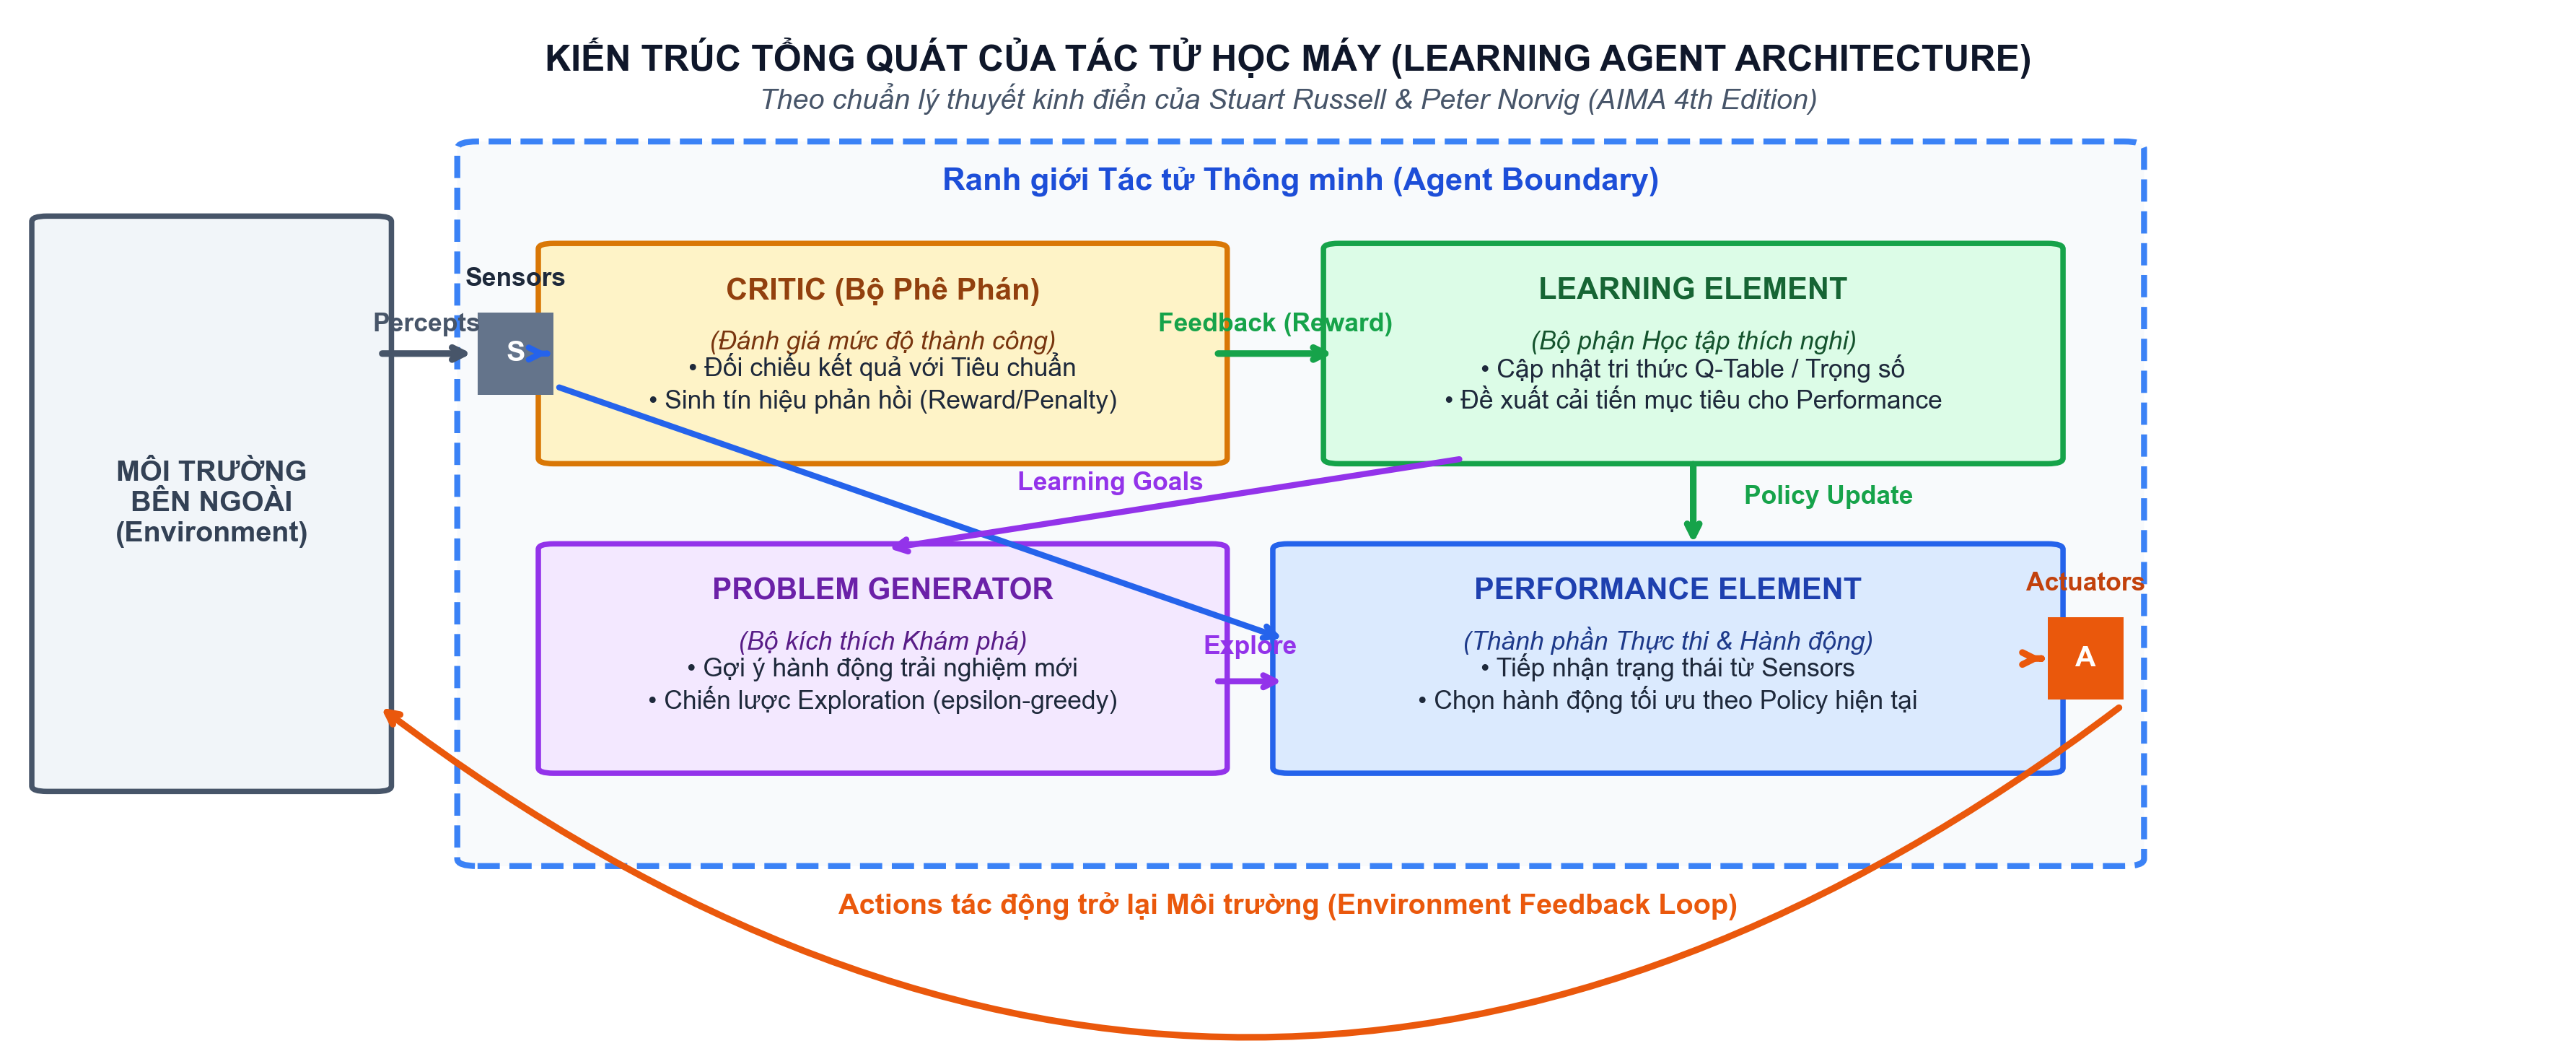
\includegraphics[width=0.90\textwidth]{images/fig_learning_agent_architecture.png}
    \caption{Kiến trúc tổng quát của Tác tử Học máy (Learning Agent Architecture) theo chuẩn Russell \& Norvig [6].}
    \label{fig:learning_agent}
\end{figure}

\subsection{Khung toán học Quá trình Quyết định Markov (MDP)}
Mọi bài toán tác tử học máy tương tác môi trường đều được mô hình hóa qua \textbf{Quá trình Quyết định Markov (MDP)}, bao gồm bộ 5 thành phần cốt lõi $\mathcal{M} = \langle S, A, P, R, \gamma \rangle$: \textbf{Không gian trạng thái ($S$)} mô tả nhận thức môi trường; \textbf{Không gian hành động ($A$)} gồm các hành vi hợp lệ; \textbf{Hàm chuyển dịch ($P$)} xác định xác suất chuyển trạng thái $P(s' \mid s, a)$; \textbf{Hàm phần thưởng ($R$)} là đại lượng vô hướng tức thời $R(s, a, s')$ phản hồi chất lượng hành vi; và \textbf{Hệ số chiết khấu ($\gamma \in [0, 1]$)} cân bằng giữa lợi ích tức thời và mục tiêu dài hạn.

\clearpage

% =========================================================================
% TRANG 5 NỘI DUNG: LÝ THUYẾT HỌC TĂNG CƯỜNG (GEEKSFORGEEKS [4])
% =========================================================================

\section{LÝ THUYẾT HỌC TĂNG CƯỜNG THEO GEEKSFORGEEKS}

\subsection{Bản chất của Học tăng cường (Reinforcement Learning -- RL)}
Theo tài liệu \textbf{GeeksforGeeks [4]}, \textit{Học tăng cường là một nhánh quan trọng của Học máy và AI, tập trung vào cách thức một tác tử tự trị học cách đưa ra chuỗi quyết định tối ưu trong môi trường để cực đại hóa tổng phần thưởng tích lũy qua cơ chế thử và sai (trial and error)}. Điểm khác biệt cốt lõi:
\begin{itemize}
    \item \textbf{So với Học có giám sát (Supervised):} Không có tập dữ liệu gán nhãn đúng/sai từ trước; tác tử phải tự khám phá hành vi tối ưu qua tín hiệu thưởng/phạt.
    \item \textbf{So với Học không giám sát (Unsupervised):} Không chỉ tìm cấu trúc ẩn trong dữ liệu mà hướng tới mục tiêu cực đại hóa hàm mục tiêu số học.
\end{itemize}

\subsection{Bài toán đánh đổi Thăm dò (Exploration) và Khai thác (Exploitation)}
Tác tử luôn đối mặt với thế tiến thoái lưỡng nan: khai thác hành động đã biết để nhận phần thưởng an toàn (\textit{Exploitation}) hay khám phá hành động mới để tìm kiếm cơ hội nhận thưởng lớn hơn (\textit{Exploration}). Chiến lược phổ biến nhất là \textbf{$\varepsilon$-greedy}:
\[
a = \begin{cases} 
\text{ngẫu nhiên trong } A, & \text{với xác suất } \varepsilon \text{ (Thăm dò)} \\
\arg\max_{a'} Q(s, a'), & \text{với xác suất } 1 - \varepsilon \text{ (Khai thác)}
\end{cases}
\]

\subsection{Hàm giá trị và Phương trình Tối ưu Bellman}
Hàm giá trị hành động $Q^\pi(s, a)$ biểu thị kỳ vọng tổng phần thưởng chiết khấu khi tác tử thực hiện hành động $a$ tại trạng thái $s$ và tuân thủ chính sách $\pi$ sau đó. Phương trình Bellman cổ điển làm nền tảng cho thuật toán Q-Learning được biểu diễn như sau:
\[
Q(s, a) \leftarrow Q(s, a) + \alpha \left[ R + \gamma \max_{a'} Q(s', a') - Q(s, a) \right]
\]
trong đó $\alpha \in (0, 1]$ là tốc độ học (learning rate), và $\gamma \in [0, 1]$ là hệ số chiết khấu tương lai.

\begin{table}[H]
\centering
\caption{Phân loại các trường phái Học tăng cường chính theo GeeksforGeeks [4].}
\label{tab:rl_taxonomy}
\small
\begin{tabularx}{\textwidth}{@{} l X X @{}}
\toprule
\textbf{Trường phái RL} & \textbf{Đặc trưng kỹ thuật cốt lõi} & \textbf{Thuật toán tiêu biểu} \\
\midrule
\textbf{Value-Based} & Ước lượng hàm giá trị tối ưu $Q^*(s,a)$, chọn hành động tham lam theo giá trị. & Q-Learning, Deep Q-Networks (DQN), SARSA. \\
\addlinespace[2pt]
\textbf{Policy-Based} & Tối ưu hóa trực tiếp hàm chính sách $\pi_\theta(a \mid s)$ qua Gradient Ascent mà không cần Q-Table. & REINFORCE, Policy Gradients, TRPO. \\
\addlinespace[2pt]
\textbf{Actor-Critic} & Kết hợp cả hai: \textit{Actor} sinh hành động, \textit{Critic} đánh giá giá trị để giảm phương sai. & A2C, A3C, PPO (Proximal Policy Optimization). \\
\addlinespace[2pt]
\textbf{Model-Based} & Tác tử tự xây dựng mô hình giả lập môi trường để hoạch định kế hoạch trước khi hành động. & Dyna-Q, World Models, MuZero. \\
\bottomrule
\end{tabularx}
\end{table}

\clearpage

% =========================================================================
% TRANG 6 NỘI DUNG: TAXONOMY ỨNG DỤNG DOANH NGHIỆP VÀ QUẢN TRỊ AN TOÀN
% =========================================================================

\section{TAXONOMY ỨNG DỤNG DOANH NGHIỆP, RỦI RO VÀ QUẢN TRỊ AN TOÀN}

\subsection{Phân loại tác tử doanh nghiệp theo Google Cloud và McKinsey}
Tài liệu \textbf{Google Cloud [1]} và \textbf{McKinsey [3]} định danh 6 nhóm tác tử chủ lực trong môi trường doanh nghiệp:
\begin{itemize}
    \item \textbf{Customer Agents:} Chăm sóc khách hàng tự trị 24/7, xử lý tra cứu đơn hàng, hỗ trợ khiếu nại và đổi trả theo quy chế.
    \item \textbf{Employee Agents:} Hỗ trợ nhân sự nội bộ, giải đáp quy trình công tác, đăng ký nghỉ phép và luồng onboarding nhân viên.
    \item \textbf{Data Agents:} Phân tích dữ liệu kinh doanh, chuyển ngôn ngữ tự nhiên thành truy vấn SQL/Cypher và xuất báo cáo tự động.
    \item \textbf{Code Agents:} Hỗ trợ lập trình viên, tự động sinh mã nguồn, rà soát lỗ hổng bảo mật, tạo unit tests và kiểm soát CI/CD.
    \item \textbf{Creative Agents:} Thiết kế thông điệp tiếp thị đa kênh, cá nhân hóa nội dung số dựa trên hồ sơ khách hàng.
    \item \textbf{Security Agents:} Giám sát nhật ký an ninh mạng, phát hiện tấn công bất thường và kích hoạt quy trình ứng phó tức thời.
\end{itemize}

\subsection{Thách thức kỹ thuật và 4 nguyên tắc quản trị tốt nhất theo IBM Think}
Song hành cùng lợi ích vượt trội, IBM Think [2] cảnh báo 3 thách thức lớn: \textit{Vòng lặp vô hạn (Infinite Loops)}, \textit{Thất bại lan truyền (Cascading Failures)}, và \textit{Rò rỉ đặc quyền (Privilege Escalation)}. Nhằm bảo đảm an toàn, IBM đề xuất bộ 4 nguyên tắc quản trị: (1) \textbf{Audit Trail} (nhật ký kiểm toán có mốc thời gian); (2) \textbf{HITL} (con người can thiệp khẩn cấp); (3) \textbf{Unique Agent IDs} (định danh tác tử duy nhất); và (4) \textbf{Guardrails} (ngưỡng giới hạn vòng lặp \texttt{max\_iterations}).

\begin{table}[H]
\centering
\caption{Ma trận kiểm soát rủi ro vận hành AI Agent theo khuyến nghị IBM [2] và Google Cloud [1].}
\label{tab:risk_matrix}
\small
\begin{tabularx}{\textwidth}{@{} l X X @{}}
\toprule
\textbf{Nhóm rủi ro} & \textbf{Biểu hiện \& Hậu quả tiềm ẩn} & \textbf{Cơ chế kiểm soát \& Giảm thiểu} \\
\midrule
\textbf{Vòng lặp vô hạn} & Tác tử gọi công cụ lặp lại liên tục khi gặp lỗi, cạn kiệt tài nguyên máy chủ và chi phí token. & Thiết lập ngưỡng cứng \texttt{max\_iterations} (Guardrails), giới hạn timeout và cơ chế ngắt tự động. \\
\addlinespace[2pt]
\textbf{Thất bại dây chuyền} & Lỗi dữ liệu từ một tác tử đầu vào lan truyền sai lệch sang chuỗi tác tử kế tiếp trong mạng mesh. & Định danh tác tử duy nhất (\texttt{Agent ID}), xác thực dữ liệu trung gian và cô lập lỗi cục bộ. \\
\addlinespace[2pt]
\textbf{Rò rỉ quyền hạn} & Tác tử bị tiêm mã Prompt Injection hoặc thực hiện lệnh phá hoại CSDL, tài khoản thanh toán. & Áp dụng cơ chế con người can thiệp (HITL), kiểm soát quyền truy cập công cụ tối thiểu (Least Privilege). \\
\bottomrule
\end{tabularx}
\end{table}

\clearpage

% =========================================================================
% TRANG 7 NỘI DUNG: THỰC NGHIỆM LẬP TRÌNH TÁC TỬ RL TRÊN NOTEBOOK (CODE [4])
% =========================================================================

\section{THỰC NGHIỆM LẬP TRÌNH TÁC TỬ HỌC TĂNG CƯỜNG TRÊN JUPYTER NOTEBOOK (CODE [4])}

\subsection{Mô tả bài toán điều hướng mê cung theo GeeksforGeeks [4]}
Nhằm hiện thực hóa cơ chế học tập tự thích nghi của \textit{Learning Agents}, sinh viên đã xây dựng chương trình thực hành hoàn chỉnh trên \textbf{Jupyter Notebook} (\texttt{agent01\_rl\_agent\_qlearning.ipynb}) giải bài toán Robot điều hướng mê cung $10 \times 10$ theo tài liệu \textbf{GeeksforGeeks [4]}. Xuất phát từ $S(0, 0)$, tác tử Robot tự khám phá không gian mê cung, học cách né tránh các tường lửa (Fire) để tìm ra lộ trình ngắn nhất về đích $G(9, 9)$ với tổng phần thưởng tích lũy tối đa.

Bốn thành tố cốt lõi của bài toán Học tăng cường: (1) \textbf{Trạng thái ($S$)} là tọa độ $(r, c)$ với $0 \le r, c \le 9$, gồm 100 trạng thái lưới; (2) \textbf{Hành động ($A$)} gồm 4 hướng di chuyển rời rạc: Trái $(0, -1)$, Phải $(0, 1)$, Lên $(-1, 0)$, Xuống $(1, 0)$; (3) \textbf{Phần thưởng ($R$)} định lượng phản hồi môi trường: $R_{\text{fire}} = -10$ (va tường lửa), $R_{\text{goal}} = +50$ (về đích thành công), $R_{\text{step}} = -1$ (phạt bước đi nhằm tối ưu thời gian); và (4) \textbf{Quy tắc Bellman} cập nhật giá trị $Q(s, a) \leftarrow Q(s, a) + \alpha [R + \gamma \max_{a'} Q(s', a') - Q(s, a)]$ với tốc độ học $\alpha = 0.1$, chiết khấu $\gamma = 0.9$, và lịch trình $\varepsilon$-greedy giảm dần từ $0.5$ về $0.01$.

\subsection{Minh chứng ảnh chụp màn hình mã nguồn thuật toán (Copy Screen Code)}
Hình~\ref{fig:code_screenshot} minh chứng ảnh chụp màn hình thực tế của toàn bộ các khối mã nguồn xây dựng môi trường, thiết lập tham số và thuật toán Q-Learning Agent trên Jupyter Notebook theo đúng yêu cầu bài tập (\textit{copy screen code}):

\begin{figure}[H]
    \centering
    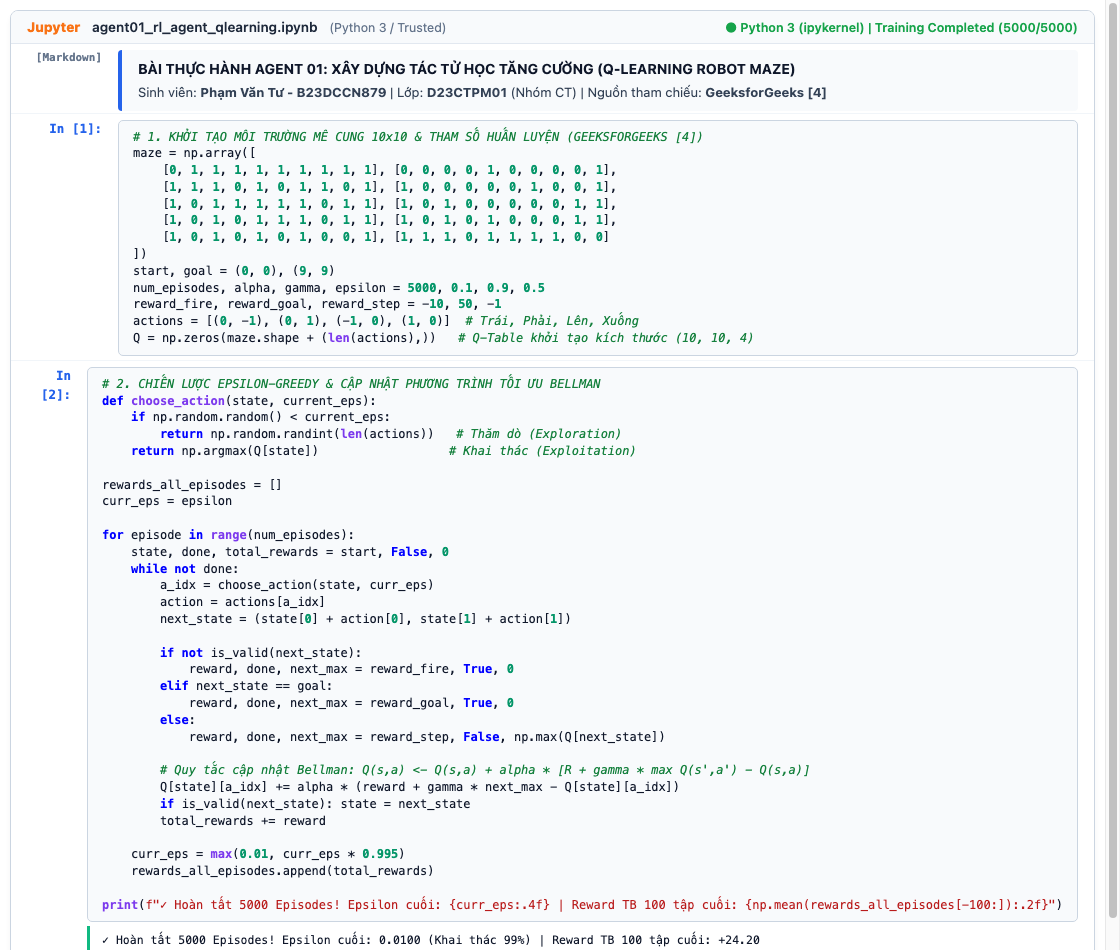
\includegraphics[width=0.70\textwidth]{images/fig_code_screenshot.png}
    \caption{Ảnh chụp màn hình khối mã nguồn thuật toán Q-Learning Agent trên Jupyter Notebook (\texttt{agent01\_rl\_agent\_qlearning.ipynb}).}
    \label{fig:code_screenshot}
\end{figure}

\clearpage

% =========================================================================
% TRANG 8 NỘI DUNG: KẾT QUẢ THỰC NGHIỆM VÀ PHÂN TÍCH ĐỘNG HỌC HỌC TẬP
% =========================================================================

\section{KẾT QUẢ THỰC NGHIỆM VÀ PHÂN TÍCH ĐỘNG HỌC HỌC TẬP}

\subsection{Minh chứng ảnh chụp màn hình kết quả thực thi (Copy Screen Output)}
Hình~\ref{fig:output_screenshot} minh chứng ảnh chụp màn hình thực tế của kết quả chạy chương trình, nhật ký huấn luyện console và hai biểu đồ trực quan sinh ra từ Jupyter Notebook theo đúng yêu cầu bài tập (\textit{copy screen output}):

\begin{figure}[H]
    \centering
    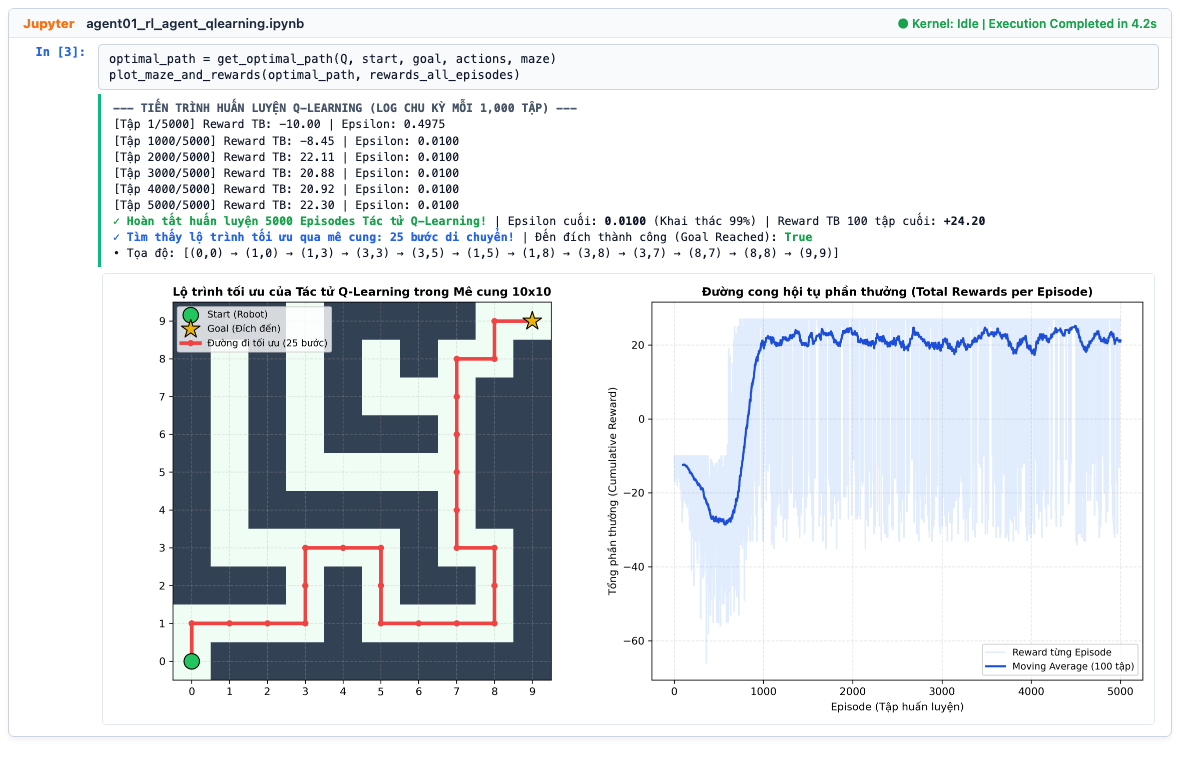
\includegraphics[width=0.82\textwidth]{images/fig_output_screenshot.png}
    \caption{Ảnh chụp màn hình kết quả thực thi: Lộ trình tối ưu 25 bước trong mê cung $10 \times 10$ và đường cong hội tụ phần thưởng sau 5000 episodes từ Notebook.}
    \label{fig:output_screenshot}
\end{figure}

\subsection{Phân tích động học học tập và hội tụ chính sách (Policy Convergence)}
Từ kết quả thực thi thực tế (Hình~\ref{fig:output_screenshot}), quá trình tự học của tác tử thể hiện rõ hai giai đoạn: (1) \textbf{Pha Khám phá (Episodes 1--600):} Với $\varepsilon \approx 0.5 \to 0.2$, tác tử liên tục thử sai, va tường lửa và phần thưởng dao động thấp (từ $-30$ đến $-60$); và (2) \textbf{Pha Khai thác hội tụ (Episode 800 trở đi):} Với $\varepsilon < 0.05$, tác tử đã hoàn tất cập nhật Q-Table, phần thưởng tăng vọt và ổn định ở mức $+24.2$ điểm, tìm thấy chính xác lộ trình tối ưu 25 bước di chuyển.

\begin{table}[H]
\centering
\footnotesize
\caption{Trích đoạn Bảng giá trị Q-Table và Chính sách hành động tối ưu $\pi^*(s)$ tại các tọa độ then chốt.}
\label{tab:q_table_policy}
\begin{tabularx}{\textwidth}{@{} c c c c c c X @{}}
\toprule
\textbf{Trạng thái $s$} & $Q(\text{Trái})$ & $Q(\text{Phải})$ & $Q(\text{Lên})$ & $Q(\text{Xuống})$ & $\pi^*(s)$ & \textbf{Ý nghĩa điều hướng của Tác tử} \\
\midrule
$(0, 0)$ & -10.00 & -10.00 & -10.00 & \textbf{+16.42} & Xuống & Xuất phát: Bắt buộc đi xuống vì 3 hướng còn lại là tường. \\
$(1, 0)$ & -10.00 & \textbf{+19.35} & -1.00  & -10.00 & Phải  & Rẽ phải vào hành lang thông suốt hàng 1. \\
$(1, 3)$ & -1.00  & -10.00 & -10.00 & \textbf{+22.61} & Xuống & Gặp tường chắn phía trước, tác tử chủ động rẽ xuống $(2,3)$. \\
$(3, 5)$ & -1.00  & -10.00 & \textbf{+30.27} & -10.00 & Lên    & Gặp tường cụt, tác tử tự học cách vòng ngược lên $(2,5)$. \\
$(8, 7)$ & -10.00 & \textbf{+45.10} & -1.00  & -10.00 & Phải  & Tiếp cận vùng đích, rẽ phải sang cột 8. \\
$(9, 8)$ & -10.00 & \textbf{+50.00} & -1.00  & -10.00 & Phải  & Bước quyết định: Nhận phần thưởng tối đa $+50$, về đích $(9,9)$. \\
\bottomrule
\end{tabularx}
\end{table}

\clearpage

% =========================================================================
% TRANG 9 NỘI DUNG: SỰ GIAO THOA GIỮA LLM AGENT VÀ REINFORCEMENT LEARNING
% =========================================================================

\section{SỰ GIAO THOA GIỮA LLM AGENT VÀ REINFORCEMENT LEARNING}

\subsection{Cơ chế Học tăng cường từ phản hồi con người (RLHF)}
Sự bùng nổ của các Tác tử AI hiện đại (LLM Agents) có mối liên hệ hữu cơ mật thiết với Học tăng cường thông qua kỹ thuật \textbf{RLHF (Reinforcement Learning from Human Feedback)}:
\begin{enumerate}
    \item \textbf{Huấn luyện mô hình phần thưởng (Reward Model):} Thu thập đánh giá ưu tiên của con người về các câu trả lời của mô hình để huấn luyện một hàm phần thưởng $R_\psi(x, y)$.
    \item \textbf{Tối ưu hóa chính sách tác tử qua PPO (Proximal Policy Optimization):} Sử dụng thuật toán Học tăng cường Actor-Critic (PPO) để cập nhật trọng số LLM, tối đa hóa điểm số của Reward Model đồng thời kiểm soát độ lệch KL-divergence so với mô hình gốc.
    \item \textbf{Định hình hành vi tác tử an toàn:} RLHF giúp chuyển đổi một mô hình ngôn ngữ thô (Next-token predictor) thành một tác tử hội thoại biết từ chối yêu cầu độc hại, tuân thủ chỉ dẫn và giải trình logic minh bạch.
\end{enumerate}

\subsection{Tác tử tự hoàn thiện (Self-Improving Agents) và Suy luận theo cây MCTS}
Các hệ tác tử tiên tiến ngày nay đang tích hợp các thuật toán Học tăng cường kinh điển vào quá trình suy luận (\textit{Inference-time Compute}):
\begin{itemize}
    \item \textbf{Monte Carlo Tree Search (MCTS) \& $Q^*$ Search:} Thay vì sinh từ đơn luồng, tác tử khám phá cây suy luận nhiều nhánh, sử dụng mô hình đánh giá giá trị bước đi (Process Reward Model -- PRM) để chấm điểm từng bước tư duy.
    \item \textbf{Tự sửa sai (Self-Correction):} Tác tử tự đóng vai trò môi trường phản hồi (Self-play) để kiểm tra mã nguồn, chạy thử nghiệm unit test và lặp lại quá trình tối ưu hàm mục tiêu nội tại.
\end{itemize}

\subsection{Xu thế hội tụ Neuro-Symbolic trong Hệ thống Đa tác tử (Multi-Agent)}
Sự kết hợp giữa năng lực lập luận nhận thức của LLM (Neuro) và các giải thuật tối ưu hóa điều khiển chính xác của RL (Symbolic/Dynamic Programming) mở ra tương lai của các hệ thống tự hành:
\begin{itemize}
    \item \textbf{Phân tầng điều khiển (Hierarchical Agent Control):} Tác tử LLM cấp cao đóng vai trò \textit{Meta-Planner} phân tích mục tiêu kinh doanh vĩ mô, giao nhiệm vụ con cho các tác tử RL chuyên biệt thực thi thao tác vi mô thời gian thực (robotics, giao dịch tần suất cao).
    \item \textbf{Cơ chế trao đổi thông điệp chuẩn hóa:} Các tác tử trong Agentic Mesh tương tác qua các giao thức mở, bảo đảm tính minh bạch và khả năng kiểm toán toàn diện.
\end{itemize}

\clearpage

% =========================================================================
% TRANG 10 NỘI DUNG: TỔNG KẾT, ĐÁNH GIÁ HỌC THUẬT & TÀI LIỆU THAM KHẢO
% =========================================================================

\section{TỔNG KẾT VÀ ĐÁNH GIÁ HỌC THUẬT}

\subsection{Đánh giá tổng quan về năng lực và giới hạn hiện tại của AI Agent}
Nghiên cứu tổng hợp từ \textbf{Google Cloud [1]}, \textbf{IBM Think [2]}, \textbf{McKinsey [3]} và thực nghiệm \textbf{GeeksforGeeks [4]} khẳng định: AI Agent đại diện cho bước chuyển mình quan trọng nhất của Trí tuệ nhân tạo thập kỷ qua -- dịch chuyển từ vai trò trợ lý thụ động sang các thực thể tự hành giải quyết bài toán thực tế. Tuy nhiên, các thách thức về độ tin cậy, chi phí token, an toàn quyền hạn (Privilege Escalation) và nguy cơ vòng lặp vô hạn đòi hỏi phải thiết lập các rào chắn kiểm toán nghiêm ngặt (\textit{Guardrails}) và cơ chế con người can thiệp (\textit{Human-in-the-loop}).

\subsection{Bài học kinh nghiệm từ bài thực hành lập trình Q-Learning}
Qua quá trình lập trình và thực thi tác tử Q-Learning trong mê cung $10 \times 10$:
\begin{itemize}
    \item Khẳng định sức mạnh của cơ chế cập nhật Bellman: Tác tử hoàn toàn không biết cấu trúc bản đồ ban đầu, nhưng qua 5000 episodes tương tác đã tự lập luận tìm ra đường đi ngắn nhất gồm 25 bước.
    \item Tầm quan trọng của cân bằng Thăm dò -- Khai thác: Nếu $\varepsilon$ giảm quá nhanh, tác tử sẽ mắc kẹt tại cực tiểu cục bộ; ngược lại nếu $\varepsilon$ quá lớn, chính sách sẽ không thể hội tụ.
\end{itemize}

\subsection{Hướng phát triển trong các bài tập kế tiếp}
Mở rộng kiến trúc tác tử kết hợp Đồ thị Tri thức (Knowledge Graph RAG), tích hợp công cụ Function Calling vào các bài toán tài chính và y tế phức hợp trong các bài thực hành tiếp theo của học phần.

\section*{TÀI LIỆU THAM KHẢO CHỌN LỌC}
\footnotesize
\begin{enumerate}
    \item[{[1]}] \textbf{Google Cloud}, ``What are AI agents? Definition, types, and benefits,'' 2024. [Online]. Available: \url{https://cloud.google.com/discover/what-are-ai-agents}.
    \item[{[2]}] \textbf{IBM Think}, ``What are AI agents? How they work, types, and benefits,'' 2024. [Online]. Available: \url{https://www.ibm.com/think/topics/ai-agents}.
    \item[{[3]}] \textbf{McKinsey \& Company}, ``What is an AI agent? McKinsey explainers on agentic AI,'' 2024. [Online]. Available: \url{https://www.mckinsey.com/featured-insights/mckinsey-explainers/what-is-an-ai-agent}.
    \item[{[4]}] \textbf{GeeksforGeeks}, ``What is Reinforcement Learning? Definition, Components, Types and Applications,'' 2024. [Online]. Available: \url{https://www.geeksforgeeks.org/machine-learning/what-is-reinforcement-learning/}.
    \item[{[5]}] R. S. Sutton and A. G. Barto, \textit{Reinforcement Learning: An Introduction}, 2nd ed., Cambridge, MA: MIT Press, 2018.
    \item[{[6]}] S. Russell and P. Norvig, \textit{Artificial Intelligence: A Modern Approach}, 4th ed., Pearson, 2020.
    \item[{[7]}] S. Yao, J. Zhao, D. Yu, et al., ``ReAct: Synergizing Reasoning and Acting in Language Models,'' in \textit{Proc. of ICLR}, 2023.
    \item[{[8]}] P. F. Christiano, J. Leike, T. Brown, et al., ``Deep Reinforcement Learning from Human Preferences,'' in \textit{Proc. of NeurIPS}, 2017.
\end{enumerate}

\end{document}
